\documentclass{beamer}
\beamertemplatenavigationsymbolsempty
\usepackage{amsmath, amssymb, hyperref, graphics}
\usepackage{tikz}

\title{Graph Theory Lecture 5}

\begin{document}
\begin{frame}{Last time: trees, ending with applications to chemistry}
\begin{block}{Review: Alkanes are trees}
  \begin{itemize}
 \item An Alkane is a molecue with formula $C_nH_{2n+2}$
 \item $3n+2$ vertices
 \item Handshaking says: $(4n+2n+2)/2=3n+1$ edges
   \item Connected, so a tree.
\end{itemize}
\end{block}

\begin{block}{Question: How many isomers does $C_5H_{12}$ have?}
  Case-by-case reasoning.  Two possible ways to organize:
  \begin{itemize}
  \item Length of longest path in carbons
  \item Highest degree just looking at carbons
    \end{itemize}
\end{block}
\end{frame}

\begin{frame}{Bridges of Konigsberg: birth of graph theory}


\begin{figure} 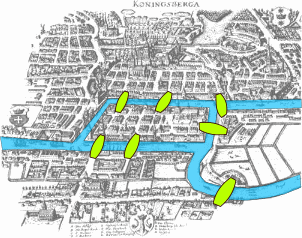
\includegraphics[width=.6\textwidth]{Pictures/Konigsberg_bridges.png} \caption{The city of Konigsberg}
\end{figure}
\begin{block}{A puzzle:}  Cross every bridge exactly once and return to where you started.
\end{block}
\end{frame}
\begin{frame}{The puzzle has no solution}
  \begin{columns}
    \begin{column}{.5\textwidth}
          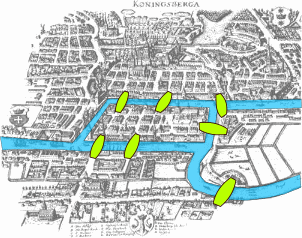
\includegraphics[width=\textwidth]{Pictures/Konigsberg_bridges.png}
      \end{column}
    \begin{column}{.5\textwidth}
      \begin{block}{Suppose there was a walk:}
      \begin{itemize}
      \item Stand on far bank
      \item Watch friend do walk
      \item Comes by one bridge
      \item Leaves by another bridge
      \item When they cross third bridge they're stuck with you
      \end{itemize}
\end{block}
      \end{column}
    \end{columns}
 \end{frame}
\begin{frame}{Generalizing with graph theory}
  \begin{definition}
    \begin{itemize}
    \item A walk is \emph{closed} if it starts and ends at the same point.
    \item A graph is \emph{Eulerian} if it has a closed walk that uses every edge exactly once
    \end{itemize}
  \end{definition}

  \begin{block}{Lemma:} If $G$ is Eulerian, then every vertex has even degree.
  \end{block}
  \begin{proof}Every time the walk visits $v$, pair the edge it arrives by with the edge it leaves by.
    \end{proof}
\end{frame}  
\begin{frame}{The first theorem in graph theory}
  \begin{theorem}[Euler] A connected graph $G$ is Eulerian if and only if every vertex of $G$ has even degree.
  \end{theorem}
  \begin{proof}
    We proved Eulerian $\implies$ even degree in last lemma. \\
    For other direction:
    \begin{itemize}
    \item Walking randomly will eventually get back to where we started (why?)
    \item Remove edges we used to get a smaller graph
    \item By induction, each connected piece is Eulerian 
    \item Glue the cycles back together
    \end{itemize}
  \end{proof}
\end{frame}





\begin{frame}{What can you draw without lifting your pen or retracing?}

  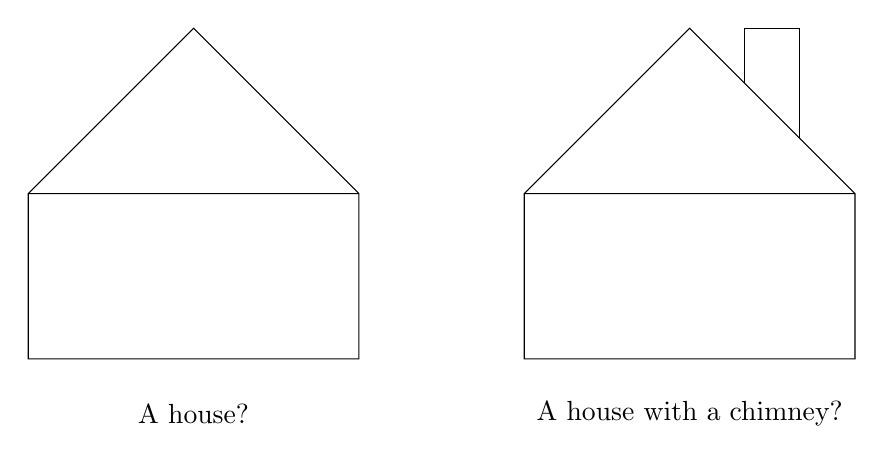
\begin{tikzpicture}[scale=.7]
    \draw (0,3)--(3,6)--(6,3)--(6,0)--(0,0)--(0,3)--(6,3);
\node at (3,-1) {A house?};


\begin{scope}[xshift=9cm]
    \draw (0,3)--(3,6)--(6,3)--(6,0)--(0,0)--(0,3)--(6,3);
    \draw (4,5)--(4,6)--(5,6)--(5,4);
\node at (3,-1) {A house with a chimney?};
\end{scope}
\end{tikzpicture}




\end{frame}

\begin{frame}{Formalizing our observations}

  \begin{definition} A graph $G$ is \emph{semi-Eulerian} if it has a (not necessarily closed) walk that uses every edge exactly once.
  \end{definition}

  \begin{theorem}A connected graph $G$ is semi-Eulerian if and only if it has at most two vertices of odd degree
  \end{theorem}
  \begin{block}{One proof: tweak the original proof}
    Easy direction: every point but start and end needs even degree. \\
    Hard direction:
    \begin{itemize}
    \item Start walk at one odd degree point
    \item Walking randomly can only end at other odd degree point
    \item Delete this path, then use induction + gluing as before
    \end{itemize}
    \end{block}


\end{frame}


\begin{frame}{A devious trick to avoid doing work}
  \begin{block}{Mathematicians are lazy}
    \begin{itemize}
      \item It's unsatisfying to ``redo'' the work of the proof  
      \item Slicker to reduce it to a problem we've already solved
    \end{itemize}
    
  \end{block}
  \begin{block}{The tricky/easy proof:}
    \begin{itemize}
    \item Let $u, v\in G$ be the two vertices of odd degree
    \item Add an edge $e$ from $u$ to $v$ to get $G^\prime$ \\
      (this may make $G$ non-simple, that's okay)
    \item In $G^\prime$, every vertex has even degree, so it has Eulerian cycle
    \item Delete $e$ from the eulerian cycle to get an Eulerian walk from $u$ to $v$
    
        \end{itemize}

    \end{block}
  

\end{frame}

\begin{frame}{A preview of next lecture}
  \begin{definition}A graph $G$ is \emph{Hamiltonian} if there is a closed walk that visits every vertex exactly once. $G$ is \emph{semi-Hamiltonian} if there is a not necessarily closed walk that visits every vertex exactly once.
  \end{definition}
  \begin{itemize}
     \item It was Easy to tell if a graph was Eulerian (Edges)
     \item It's Hard to tell if a general graph is Hamiltonian (Vertices)
  \end{itemize}
  \begin{columns}
     \begin{column}{.5\textwidth}
        \begin{block}{Question to lead into it:}
          \begin{itemize}
          \item     Is $D_{20}$ Hamiltonian?
          \item Is the Petersen graph?  
\item     If we remove a vertex from $D_{20}$ is it Hamiltonian? How about Petersen?
  \end{itemize}
        \end{block}
     \end{column}
     \begin{column}{.5\textwidth}
\begin{center}    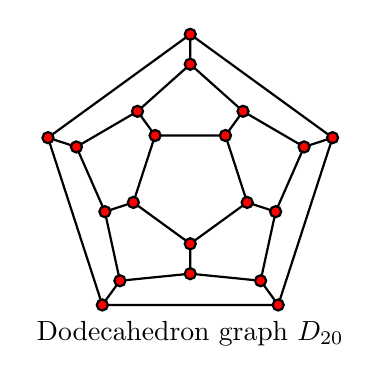
\begin{tikzpicture}[scale=.38]
            \node at (0,-5) {Dodecahedron graph $D_{20}$};       

 \begin{scope}[thick, every node/.style={draw, circle, fill=red, inner sep=0pt, minimum width=4pt} ]  
    \draw \foreach \x in {0,72,...,288}
    {
        (\x-90:2) node {}  -- (\x-18:2)
      (\x-90:2) -- (\x-90:3)
      (\x-90:3) -- (\x-54:4)
      (\x-90:3) node {} -- (\x-126:4)
      (\x+90:4) node {} -- (\x+90:5)
      (\x+90:5) node {} -- (\x+18:5)
     };
   \end{scope}
 \end{tikzpicture}\end{center}
  \end{column}
\end{columns}
\end{frame}
\end{document}
